\clearpage
\section{Real Robot Experiment}
\label{sec:appx_real_robot}

\begin{figure*}
    \centering
    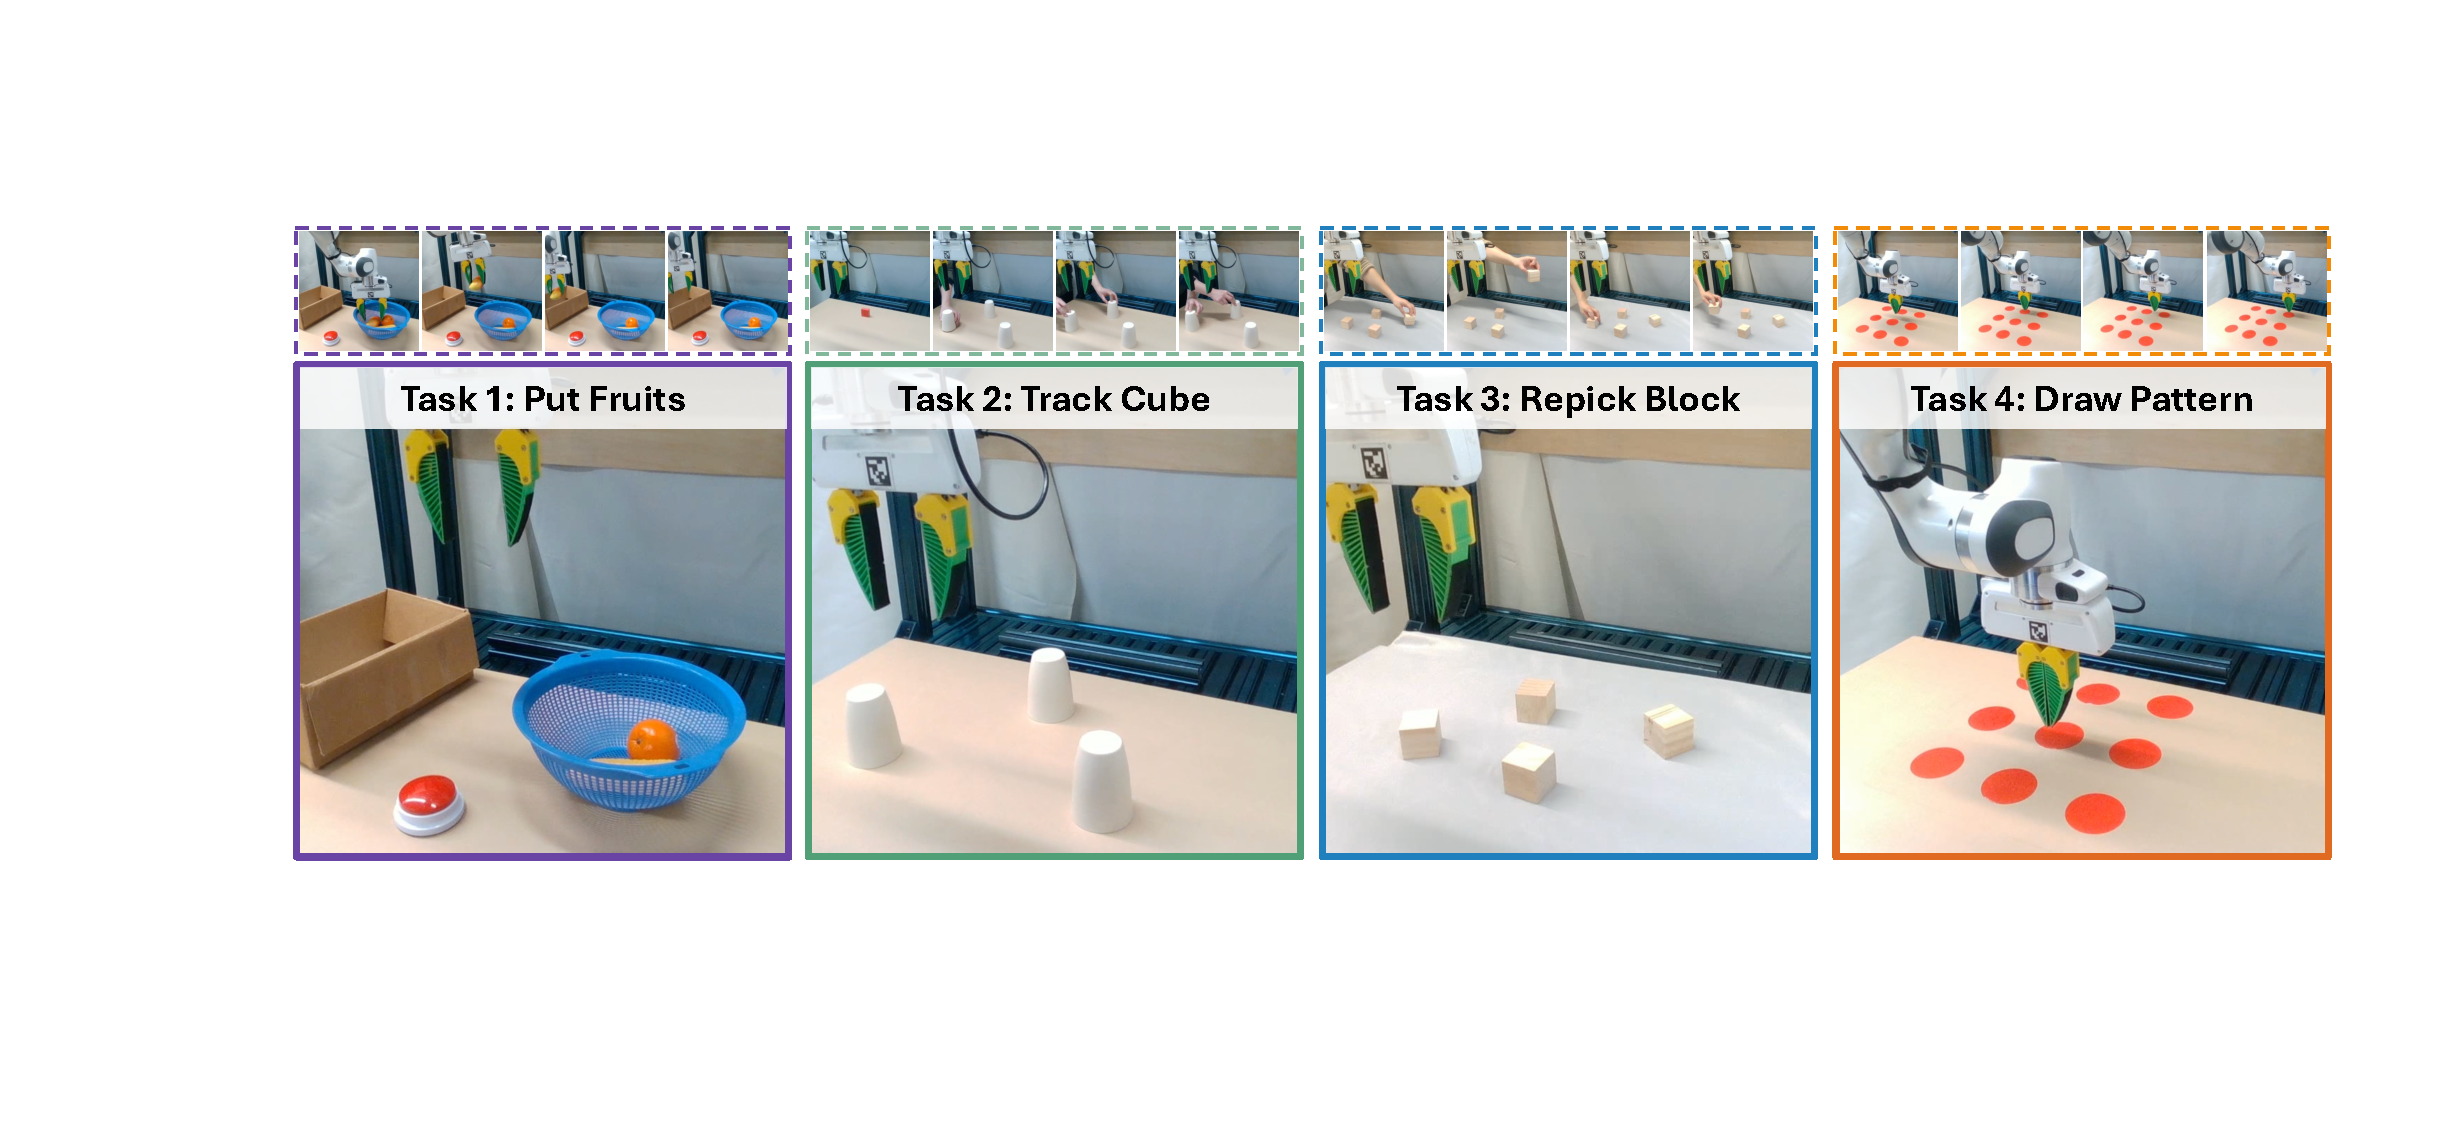
\includegraphics[width=\linewidth]{images/real_world_tasks.pdf}
    \caption{We design four history-dependent real-world tasks for policy evaluation. The upper dashed box indicate selected frames from previous video history. The bottom large box indicate current observation for execution.}
    \label{fig:real_robot}
\end{figure*}

We design four real-world tasks (Figure~\ref{fig:real_robot}), \textit{PutFruits}, \textit{TrackCube}, \textit{RepickBlock}, and \textit{DrawPattern}, to mirror four simulation tasks, \textit{BinFill}, \textit{VideoUnmask(Swap)}, \textit{VideoRepick}, and \textit{PatternLock}, respectively.
\begin{itemize}
\item \textbf{\textit{PutFruits}.} The robot transfers a specified number of fruits from a basket to a bin. During execution, a human may intervene by removing placed fruits or adding new ones, preventing the robot from relying solely on immediate perception and requiring it to track progress over time.

\item \textbf{\textit{TrackCube}.} The robot selects the correct cup containing a target cube given a pre-recorded video in which a human covers the cubes with multiple cups and optionally swaps or moves their positions.

\item \textbf{\textit{RepickBlock}.} Given a pre-recorded video showing a human picking up several blocks, the robot must identify and pick up the same set of blocks again.

\item \textbf{\textit{DrawPattern}.} The robot reproduces a movement trajectory demonstrated in a pre-recorded video.
\end{itemize}

We teleoperate the robot using an Oculus Quest~2 and record demonstrations at 15 Hz. We collect 50 demonstrations for \textit{PutFruits} and 100 demonstrations for each of the other three tasks, as \textit{PutFruits} episodes contain longer trajectories. In total, the dataset comprises 350 demonstrations and 78{,}400 timesteps.

After data collection, we manually annotate each episode with grounded subgoals at keyframes. For simplicity, we omit grounding annotations for \textit{PutFruits}, as we found that simple goal descriptions are sufficient for counting-based behaviors.
Figure~\ref{fig:platform} illustrates the platform setup. Experiments are conducted using a 7-DoF Franka Emika Panda robot equipped with UMI~\cite{chi2024UMI} fin-ray fingers mounted on the default Franka gripper. The robot operates in a tabletop environment with three RGB-D cameras following the DROID setup~\cite{khazatsky2024droid}: two Intel RealSense D435 cameras mounted on the left and right shoulders and one Intel RealSense D405 mounted on the wrist.

To assess whether the trends observed on \benchname\xspace transfer to physical settings, we evaluate our strongest perceptual model (\textsc{FrameSamp}+\texttt{Modul}), symbolic model (\textsc{GroundSG}+\texttt{QwenVL}), and the $\pi_{0.5}$ baseline for comparison. We adopt a larger memory budget of $B=2048$, as simulation experiments showed only modest additional computational cost. We use the right-shoulder view image for the VLM subgoal predictor and memory contruction.
\texttt{QwenVL} is trained using the same configuration as in simulation. The subgoal annotation for \textit{PutFruits} and \textit{DrawPattern} tasks does not contain grounding information.
All other hyperparameters remain unchanged, except that we set the total number of training steps to 50k.

\begin{figure}[t]
    \centering
    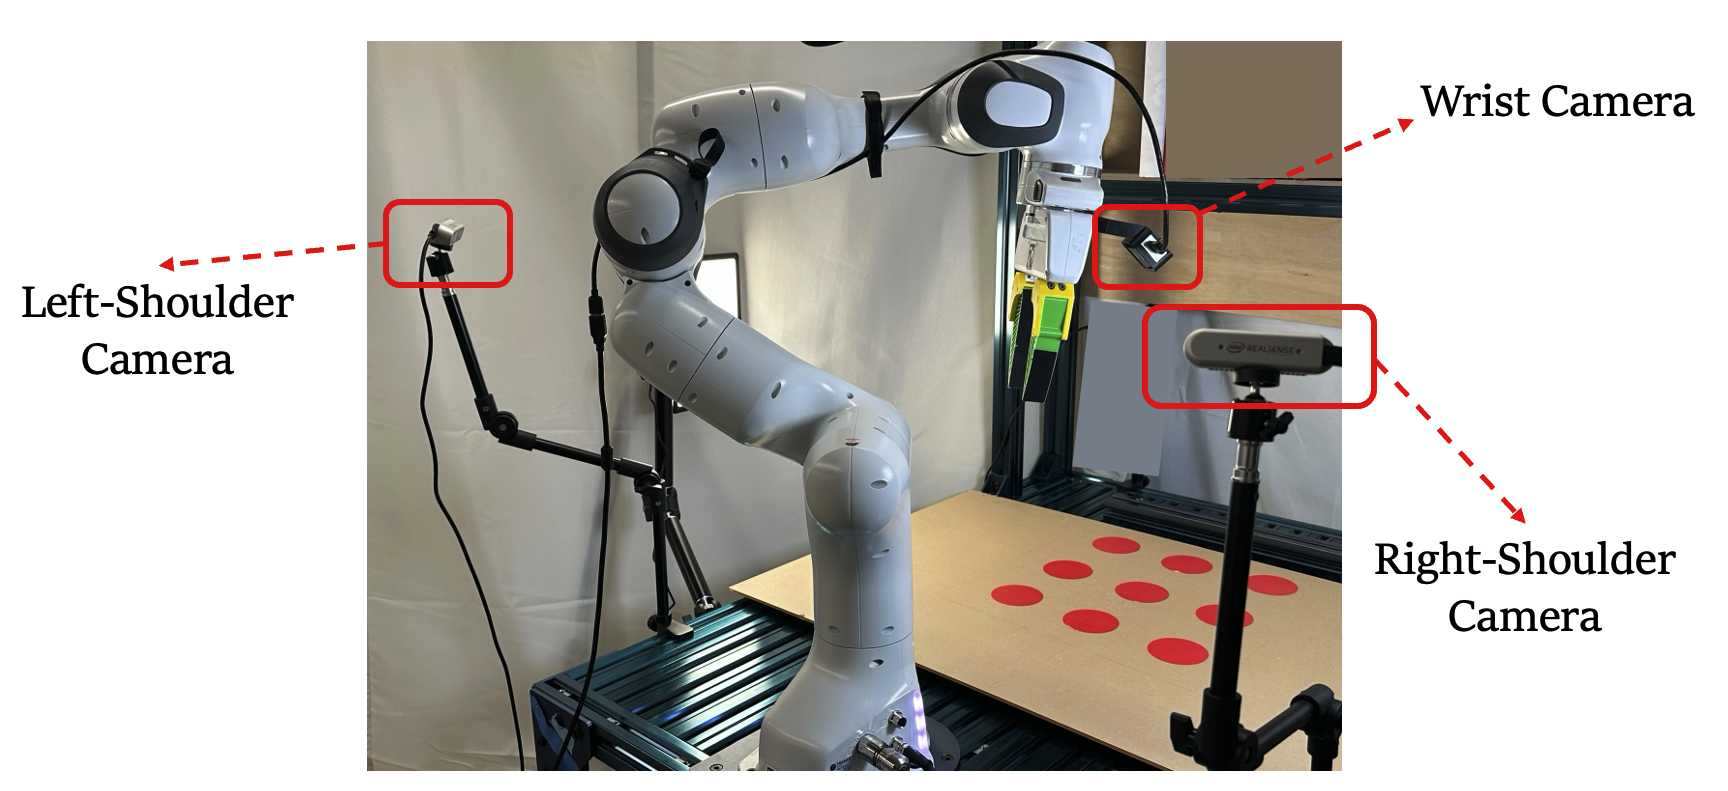
\includegraphics[width=0.8\linewidth]{images/real_robot_setup.png}
    \caption{Real Robot Experiment Platform Setup.}
    \label{fig:platform}
\end{figure}

\begin{table}[t]
    \centering
    \setlength{\tabcolsep}{3pt}
    \renewcommand{\arraystretch}{0.95}
    \resizebox{\linewidth}{!}{
    \begin{tabular}{l llll c}
\toprule
\textbf{Method} &
\makecell[l]{{\textbf{Put}} \\ {\textbf{Fruits}}} &
\makecell[l]{{\textbf{Track}} \\{\textbf{Cube}}}  &
\makecell[l]{{\textbf{Repick}} \\ {\textbf{Block}}} &
\makecell[l]{{\textbf{Draw}} \\ {\textbf{Pattern}}} &
\textbf{\texttt{Total}} \\
\midrule

$\pi_{0.5}$
& 2/10 & 1/10 & 1/10 & 0/10 & 4/40 \\

\midrule

\textsc{GroundSG} + \texttt{QwenVL}
& \best{9/10} & 3/10 & 5/10 & 2/10 & 19/40 \\

\midrule

\textsc{FrameSamp} + \texttt{Modul}
& 6/10 & \best{5/10} & \best{6/10} & \best{8/10} & \best{25/40} \\

\bottomrule
\end{tabular}
    }
    \caption{Real-world experiment results.}
    \label{tab:real}
\end{table}

The aggregated results for each task are shown in Table~\ref{tab:real}. All rollout demonstrations are available on the project website.

We observe similar trends in the real world. Perceptual memory performs best on the motion-centric task \textit{DrawPattern}, whereas symbolic memory performs better on the event-salient task \textit{PutFruits}. Both approaches achieve moderate performance on \textit{RepickBlock}. On \textit{TrackCube}, perceptual memory performs slightly better, as the VLM-based subgoal predictor often fails to produce accurate grounding when dynamic swapping occurs. Although both representations transfer the simulation trends to the real world, absolute success rates leave clear headroom on \textit{TrackCube} and \textit{RepickBlock}, suggesting room for further improvement.
